% ====================================================
%  PicoSoC 移植与验证进展汇报 — 组会 PPT
%  Author: 葛良晨
%  Date: 2026-05-21
%  Compile: latexmk -xelatex -shell-escape
% ====================================================
\documentclass[aspectratio=169, 10pt, UTF8]{ctexbeamer}

\usetheme{Madrid}
\usecolortheme{default}

\definecolor{ieeeBlue}{RGB}{0, 83, 159}
\definecolor{ieeeRed}{RGB}{198, 38, 46}
\definecolor{ieeeGreen}{RGB}{0, 114, 41}
\definecolor{ieeeOrange}{RGB}{235, 110, 31}
\definecolor{darkGray}{RGB}{66, 66, 66}

\setbeamercolor{structure}{fg=ieeeBlue}
\setbeamercolor{alerted text}{fg=ieeeRed}
\setbeamercolor{example text}{fg=ieeeGreen}
\setbeamercolor{frametitle}{bg=ieeeBlue!15, fg=ieeeBlue}
\setbeamercolor{block title}{bg=ieeeBlue!15, fg=ieeeBlue}
\setbeamercolor{block body}{bg=ieeeBlue!5}
\setbeamercolor{block title example}{bg=ieeeGreen!15, fg=ieeeGreen}
\setbeamercolor{block body example}{bg=ieeeGreen!5}
\setbeamercolor{block title alerted}{bg=ieeeRed!15, fg=ieeeRed}
\setbeamercolor{block body alerted}{bg=ieeeRed!5}

\usepackage{graphicx}
\usepackage{booktabs}
\usepackage{tabularx}
\usepackage[table]{xcolor}
\usepackage{amsmath,amssymb}
\usepackage{tikz}
\usetikzlibrary{positioning, calc, shapes.geometric, arrows.meta, backgrounds, fit}
\usepackage{hyperref}

\graphicspath{{/Volumes/mac_db/latex_prjs/riscv_doc/out/}{./assets/}}

\setbeamertemplate{footline}[frame number]

\title[PicoSoC 移植进展]{PicoSoC 移植与验证进展汇报}
\subtitle{基于 RISC-V 的 SoC：C 固件、AXI-Lite 外设驱动与 FPGA 验证}
\author[葛良晨]{葛良晨}
\institute[组会汇报]{组会汇报}
\date{2026年5月21日}

\begin{document}

\begin{frame}
  \titlepage
\end{frame}

% ============================================
\begin{frame}{项目背景与进展概览}
  \begin{columns}[T]
    \begin{column}{0.50\textwidth}
      \begin{block}{项目目标}
        \begin{itemize}
          \item 基于 PicoRV32 (RV32IMC) 构建完整 SoC
          \item AXI4-Lite 总线统一连接外设
          \item C 语言固件开发与设备驱动
          \item FPGA 原型验证
        \end{itemize}
      \end{block}
    \end{column}
    \begin{column}{0.50\textwidth}
      \begin{exampleblock}{当前进展 \checkmark}
        \begin{enumerate}
          \item SoC 集成：CPU + AXI4-Lite + 外设
          \item C 工具链：GCC + Linker + 启动代码
          \item 外设驱动：UART / SPI / BRAM / GPIO
          \item FPGA 验证：UART 输出, GPIO LED
          \item 仿真验证：SPI 全双工传输
        \end{enumerate}
      \end{exampleblock}
    \end{column}
  \end{columns}
\end{frame}


% ============================================
\begin{frame}{DC 综合资源统计}
  \begin{columns}[T]
    \begin{column}{0.52\textwidth}
      \begin{table}[h]
        \centering
        \footnotesize
        \begin{tabular}{lr}
          \toprule
          \textbf{指标} & \textbf{数量} \\
          \midrule
          Leaf Cell (叶子单元) & $\sim$47,000 \\
          Sequential Cells (时序) & $\sim$35,600 \\
          Combinational Cells (组合) & $\sim$11,400 \\
          Buf/Inv Cells & 2,291 \\
          \quad Buf & 1,357 \\
          \quad Inv & 934 \\
          Hierarchical Cells & 182 \\
          Cell Types (References) & 13 种 \\
          Nets (线网) & $\sim$59,000 \\
          Ports (端口) & $\sim$8,800 \\
          \bottomrule
        \end{tabular}
      \end{table}
    \end{column}
    \begin{column}{0.48\textwidth}
      \begin{alertblock}{关键瓶颈：SRAM 推断为寄存器阵列}
        \texttt{sram\_1rw\_wrapper} (4 KiB BRAM) 行为级模型被 DC 推断为触发器阵列：
        \[
        1024 \times 32\text{ bits} \approx 32\text{K flip-flops}
        \]
        $\Rightarrow$ 约 \textbf{90\%} 时序单元来自 SRAM 寄存器推断
      \end{alertblock}

      \begin{exampleblock}{去掉 SRAM 后（逻辑部分估算）}
        \footnotesize
        \begin{tabular}{lr}
          \toprule
          \textbf{类型} & \textbf{数量} \\
          \midrule
          逻辑触发器 (CPU + 外设) & $\sim$3,600 \\
          组合逻辑单元 & $\sim$11,400 \\
          总逻辑单元 (GTECH) & $\sim$15,000 \\
          \bottomrule
        \end{tabular}
      \end{exampleblock}
    \end{column}
  \end{columns}

  \vspace{4pt}
  \begin{center}
    {\footnotesize\color{ieeeRed} 真实 ASIC 应将 SRAM 替换为 Memory Compiler 宏（面积可减少 10--50$\times$）}
  \end{center}
\end{frame}

% ============================================
\begin{frame}{TSMC 28nm HPC+ 综合结果}
  \begin{center}
    {\footnotesize \texttt{tcbn28hpcplusbwp40p140ssg0p72v125c\_ccs}}
  \end{center}

  \begin{columns}[T]
    \begin{column}{0.48\textwidth}
      \begin{table}[h]
        \centering
        \footnotesize
        \begin{tabular}{lr}
          \toprule
          \textbf{指标} & \textbf{数量} \\
          \midrule
          Ports & 2,075 \\
          Nets & 105,964 \\
          Cells (总计) & 104,343 \\
          \quad Combinational & 68,918 \\
          \quad Sequential & 35,415 \\
          \quad Buf/Inv & 1,712 \\
          References & 24 种 \\
          \bottomrule
        \end{tabular}
      \end{table}
    \end{column}
    \begin{column}{0.52\textwidth}
      \begin{table}[h]
        \centering
        \footnotesize
        \begin{tabular}{lr}
          \toprule
          \textbf{面积} & \textbf{数值} \\
          \midrule
          Combinational area & 45,949.68 \\
          Noncombinational area & 67,028.60 \\
          Buf/Inv area & 486.23 \\
          \rowcolor{ieeeRed!10}
          Total cell area & \textbf{112,978.28} \\
          \bottomrule
        \end{tabular}
      \end{table}
    \end{column}
  \end{columns}

  \vspace{6pt}
  \begin{block}{层次化面积分布}
    \centering
    \footnotesize
    \begin{tabular}{lrr}
      \toprule
      \textbf{模块} & \textbf{面积} & \textbf{占比} \\
      \midrule
      \rowcolor{ieeeRed!12}
      \texttt{sram\_u} (SRAM 4 KiB) & 102,419.48 & 90.7\% \\
      \texttt{cpu\_axi/picorv32\_core} & 9,447.23 & 8.4\% \\
      \quad \texttt{pcpi\_mul} & 948.15 & 0.8\% \\
      \quad \texttt{pcpi\_div} & 908.33 & 0.8\% \\
      \texttt{uart\_axi} & 647.64 & 0.6\% \\
      \texttt{dsp\_axi} & 256.66 & 0.2\% \\
      \texttt{sram\_bridge} & 104.08 & 0.1\% \\
      \texttt{cpu\_axi/axi\_adapter} & 17.26 & $<$0.1\% \\
      \bottomrule
    \end{tabular}
  \end{block}

  \vspace{2pt}
  \begin{center}
    {\footnotesize\color{ieeeRed} SRAM 仍占 90.7\% 面积，替换为 Memory Compiler 宏后逻辑部分仅 $\sim$10.5K 面积单位}
  \end{center}
\end{frame}

% ============================================
\begin{frame}{PicoSoC 系统架构总览}
  \centering
  \includegraphics[width=0.88\textwidth, height=0.78\textheight, keepaspectratio]{diagram_v2.pdf}
\end{frame}

% ============================================
\begin{frame}{地址空间布局 (Memory Map)}
  \centering
  \includegraphics[width=0.52\textwidth, height=0.72\textheight, keepaspectratio]{picosoc_memory_map.pdf}

  \vspace{5pt}
  \begin{columns}[T]
    \begin{column}{0.30\textwidth}
      \centering \textbf{0x0000\_0000}\\{\footnotesize Internal SRAM (16 MiB)}
    \end{column}
    \begin{column}{0.30\textwidth}
      \centering \textbf{0x0100\_0000}\\{\footnotesize XIP SPI Flash (16 MiB)}
    \end{column}
    \begin{column}{0.30\textwidth}
      \centering \textbf{0x0200\_0000}\\{\footnotesize MMIO: UART/SPI/GPIO}
    \end{column}
  \end{columns}
\end{frame}

% ============================================
\begin{frame}{AXI4-Lite SPI Master 架构}
  \centering
  \includegraphics[width=0.75\textwidth, height=0.78\textheight, keepaspectratio]{spi_master.pdf}
\end{frame}

% ============================================
\begin{frame}{设备驱动概览}
  \begin{table}[h]
    \centering
    \footnotesize
    \begin{tabular}{lllp{0.42\textwidth}}
      \toprule
      \textbf{外设} & \textbf{基地址} & \textbf{关键寄存器} & \textbf{驱动功能} \\
      \midrule
      \rowcolor{ieeeBlue!5}
      UART  & 0x0200\_0000 & DAT, DIV      & 串口收发, printf 格式化输出 \\
      \rowcolor{ieeeGreen!5}
      SPI   & 0x0200\_0100 & CTRL, TX\_MEM, RX\_MEM & 全双工传输, CPOL/CPHA 配置 \\
      \rowcolor{ieeeOrange!5}
      GPIO  & 0x0200\_0200 & OUT, DIR, IN  & LED 控制, 按键输入 \\
      \rowcolor{ieeeRed!5}
      BRAM  & 0x0000\_0000 & —             & C 指针直接读写 SRAM \\
      \bottomrule
    \end{tabular}
  \end{table}

  \begin{itemize}
    \item 外设统一编址在 AXI4-Lite 总线上，CPU 通过 load/store 指令访问
    \item C 驱动通过 volatile 指针映射外设寄存器地址
    \item MMR 寄存器 RTL 由 Python 脚本自动生成
  \end{itemize}
\end{frame}

% ============================================
\begin{frame}{C 固件结构与构建流程}
  \begin{columns}[T]
    \begin{column}{0.48\textwidth}
      \begin{block}{固件内存布局}
        \begin{itemize}
          \item \texttt{.text}  — XIP Flash (0x0100\_0000)
          \item \texttt{.rodata} — XIP Flash
          \item \texttt{.data}   — SRAM (初始化数据)
          \item \texttt{.bss}    — SRAM (零初始化)
          \item \texttt{.stack}  — SRAM 顶部向下增长
        \end{itemize}
      \end{block}
    \end{column}
    \begin{column}{0.48\textwidth}
      \begin{exampleblock}{构建流程}
        C 源码 $\xrightarrow{\text{riscv32-gcc}}$ ELF $\xrightarrow{\text{objcopy}}$ BIN
        $\xrightarrow{\text{烧录}}$ SPI Flash $\xrightarrow{\text{XIP}}$ 执行
      \end{exampleblock}

      \begin{block}{工具链}
        \begin{itemize}
          \item riscv32-unknown-elf-gcc
          \item 定制 Linker Script (.ld)
          \item 汇编启动代码 (crt0.S)
        \end{itemize}
      \end{block}
    \end{column}
  \end{columns}
\end{frame}

% ============================================
\begin{frame}{SPI 仿真验证}
  \begin{columns}[T]
    \begin{column}{0.45\textwidth}
      \begin{block}{测试用例}
        \begin{enumerate}
          \item 单字节写 (SPI Mode 0)
          \item 单字节读 (SPI Mode 0)
          \item 多字节连续传输 (8/16/32B)
          \item 四种 SPI 模式 (Mode 0/1/2/3)
          \item 多时钟分频 (div=2/4/8/16)
          \item 多片选控制 (CS[0:3])
        \end{enumerate}
      \end{block}

      \begin{exampleblock}{仿真结果}
        所有测试用例通过。SPI Master @ 50 MHz sysclk,
        div=4 (12.5 MHz SCLK), MISO/MOSI 数据比对正确。
      \end{exampleblock}
    \end{column}
    \begin{column}{0.55\textwidth}
      \centering
      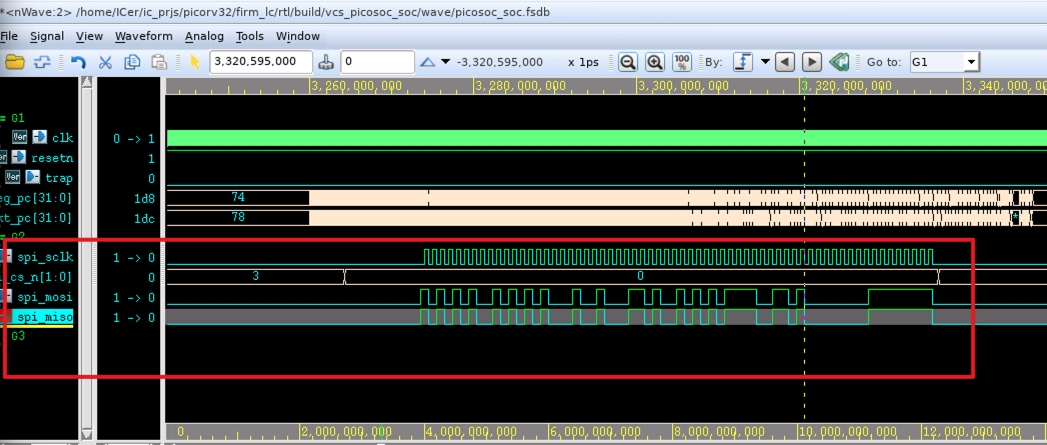
\includegraphics[width=\textwidth, height=0.72\textheight, keepaspectratio]{spi_waveform_verdi.jpg}
    \end{column}
  \end{columns}
\end{frame}

% ============================================
\begin{frame}{SPI 仿真波形：串口日志}
  \centering
  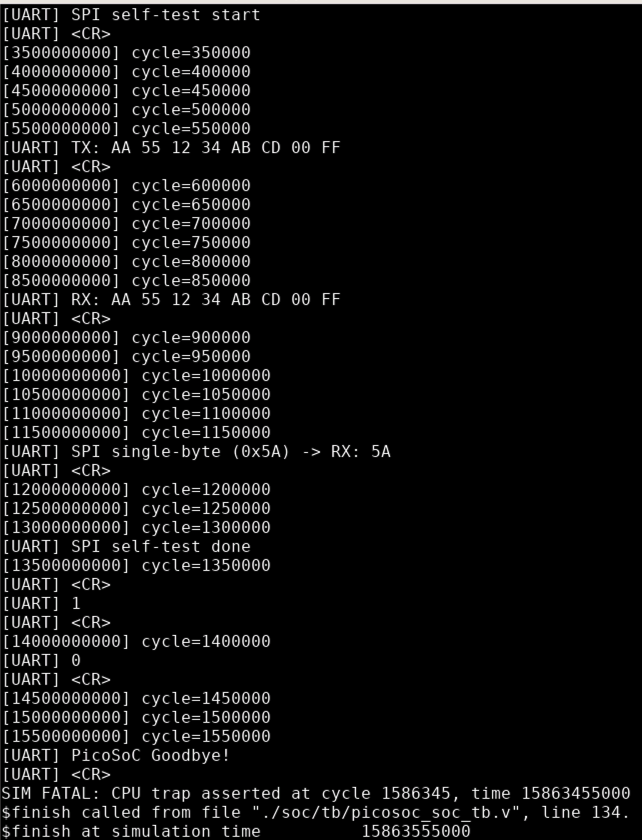
\includegraphics[width=0.92\textwidth, height=0.78\textheight, keepaspectratio]{spi_waveform_console.png}
\end{frame}

% ============================================
\begin{frame}{进展总结与后续计划}
  \begin{columns}[T]
    \begin{column}{0.50\textwidth}
      \begin{table}[h]
        \centering
        \footnotesize
        \begin{tabular}{lc}
          \toprule
          \textbf{模块} & \textbf{状态} \\
          \midrule
          \rowcolor{ieeeGreen!12}
          PicoSoC 系统集成 & \checkmark 完成 \\
          \rowcolor{ieeeGreen!12}
          C 固件工具链   & \checkmark 完成 \\
          \rowcolor{ieeeGreen!12}
          UART 驱动 (FPGA) & \checkmark 完成 \\
          \rowcolor{ieeeGreen!12}
          GPIO/LED 驱动   & \checkmark 完成 \\
          \rowcolor{ieeeGreen!12}
          SPI 驱动 (仿真)  & \checkmark 完成 \\
          \rowcolor{ieeeGreen!12}
          BRAM 内存访问   & \checkmark 完成 \\
          \rowcolor{ieeeOrange!8}
          SPI FPGA 实测   & 进行中 \\
          \rowcolor{ieeeOrange!8}
          I2C/Timer 外设  & 规划中 \\
          \bottomrule
        \end{tabular}
      \end{table}
    \end{column}
    \begin{column}{0.50\textwidth}
      \begin{block}{后续工作}
        \begin{enumerate}
          \item SPI 外围设备 FPGA 联调
          \item I2C Master 控制器开发
          \item Timer / PWM 硬件模块
          \item 中断控制器 (PLIC)
          \item JTAG 调试接口
          \item ASIC 后端流程评估
        \end{enumerate}
      \end{block}
    \end{column}
  \end{columns}
\end{frame}

% ============================================
\begin{frame}{PicoRV32 资源消耗 (官方数据)}
  \begin{center}
    {\footnotesize Xilinx 7-Series FPGA, area-optimized synthesis}
  \end{center}
  \begin{table}[h]
    \centering
    \footnotesize
    \begin{tabular}{lrrr}
      \toprule
      \textbf{Core Variant} & \textbf{Slice LUTs} & \textbf{LUTs as Memory} & \textbf{Slice Registers} \\
      \midrule
      \rowcolor{ieeeGreen!12}
      PicoRV32 (small)   & 761  & 48 & 442  \\
      \rowcolor{ieeeBlue!8}
      PicoRV32 (regular) & 917  & 48 & 583  \\
      \rowcolor{ieeeOrange!12}
      PicoRV32 (large)   & 2019 & 88 & 1085 \\
      \bottomrule
    \end{tabular}
  \end{table}

  \begin{itemize}
    \item \textbf{small} — 无 CSR 指令、无两级移位、mem\_rdata 外部锁存、不捕获非对齐访问与非法指令
    \item \textbf{regular} — 默认配置，面积/性能平衡
    \item \textbf{large} — 开启 PCPI、IRQ、MUL、DIV、BARREL\_SHIFTER、COMPRESSED\_ISA
  \end{itemize}
\end{frame}
% ============================================
\begin{frame}[plain]
  \centering
  \vfill
  {\huge\color{ieeeBlue} 谢谢！欢迎提问与讨论}

  \vspace{20pt}
  {\large 葛良晨}

  \vspace{8pt}
  {\normalsize 2026年5月21日}
  \vfill
\end{frame}

\end{document}
